% ============================================================
% Decision Level Sensor Fusion for Home Fall Monitoring
% IEEE conference format (IEEEtran). Compiles on Overleaf as is.
% ============================================================
\documentclass[conference]{IEEEtran}
\usepackage{amsmath,amssymb}
\usepackage{graphicx}
\usepackage{booktabs}
\usepackage{array}
\usepackage{textcomp}
\usepackage{xcolor}
\IEEEoverridecommandlockouts

\begin{document}

\title{Decision Level Sensor Fusion for Home Fall Monitoring:\\
A Co Observed Leaderboard Evaluation}

\author{\IEEEauthorblockN{Rudra Chopra}
\IEEEauthorblockA{
San Ramon, California, USA\\
Email: rudrachopra023@gmail.com}}

\maketitle

\begin{abstract}
Home fall monitoring systems often rely on a single sensing stream. A camera
can mistake sitting, lying down, or bending for a fall, and a body worn motion
sensor can react to benign movement or signal artifacts. This paper studies
decision level fusion: a camera detector and an accelerometer detector are
trained and run independently, and a decision layer combines their current and
recent outputs. We evaluate on the UR Fall Detection Dataset, in which a camera
and a body worn accelerometer recorded the same falls at the same time, so the
joint structure between the streams and the temporal continuity within each
sequence are real rather than constructed. Across 70 sequences and 11{,}505 co
observed frames we benchmark fourteen decision layers, from single sensors and
simple score combiners through rule based agreement rules to learned fusion
models. A learned temporal fusion, a logistic model over causal temporal
features of the two score streams, is the strongest method: it reaches an F1 of
0.863 against 0.842 for the best single sensor, and the advantage is
statistically significant at every tested stress level (paired Wilcoxon $p$
approximately 0.002, winning all ten splits at most levels). Its false alert
rate is comparable to the camera detector. The gain is modest, roughly two to
three F1 points, and it comes from the learned model: a hand designed rule based
agreement fusion does not beat the single sensor, and equal weight score
averaging does not either. We conclude that a learned temporal decision layer
gives a small but consistent and significant improvement over the best single
sensor, while simpler fusion strategies do not, and we report this honestly
including where fusion fails to help.
\end{abstract}

\begin{IEEEkeywords}
Home monitoring, decision level fusion, fall detection, sensor fusion, temporal
modeling, robustness, co observed data.
\end{IEEEkeywords}

\section{Introduction}
Falls are a leading cause of injury and loss of independence among older
adults, and the time between a fall and assistance strongly affects outcomes.
Home monitoring systems aim to shorten that time by detecting falls
automatically. A camera provides visual evidence of body posture and motion,
while a body worn sensor provides evidence of impact and movement dynamics.
These streams are complementary, but neither is reliable enough to use alone in
every situation. A visual detector can confuse sitting, lying down, bending, or
fast movement with a fall. A motion sensor can react to vigorous but benign
activity, to sensor artifacts, or to the device being set down.

This paper studies a practical decision level design. Two detectors, one for the
camera stream and one for the accelerometer stream, are trained and run
independently. A decision layer then combines their current and recent alert
outputs. The goal is not a single end to end synchronized multimodal model. The
goal is to make monitoring decisions from independent detector outputs, which is
realistic because home sensors operate at different rates and a deployable
system should tolerate imperfect alignment.

A central difficulty in evaluating any fusion layer is data. To measure whether
combining two streams helps, the evaluation needs events in which both streams
observed the same situation, so that a real fall tends to appear on both streams
while an isolated sensor artifact appears on only one. We use the UR Fall
Detection Dataset \cite{kwolek2014}, in which a camera and an accelerometer
recorded the same real falls simultaneously. The joint structure between the
streams is therefore real and intrinsic, and each sequence is one continuous
recording, so the temporal features are computed on genuinely consecutive
frames.

We benchmark fourteen decision layers and report the result honestly. A learned
temporal fusion, a logistic model over causal temporal features of the two
detector streams, modestly but significantly and consistently outperforms the
best single sensor. Simpler fusion strategies do not: a hand designed rule based
agreement rule and equal weight score averaging both fail to beat the single
camera detector. The improvement from the learned layer is real but small, and
we are explicit about its size and about the methods that do not help.

The contributions are as follows. First, a decision level home monitoring
framework that treats the camera and accelerometer detectors as independent
alert sources combined by a decision layer. Second, a fourteen method
leaderboard on co observed camera and accelerometer fall data, spanning single
sensors, simple score combiners, rule based agreement rules, and learned fusion
models, under a controlled sensor stress protocol. Third, an honest
characterization: a learned temporal decision layer gives a small, consistent,
statistically significant gain over the best single sensor, while hand designed
and equal weight fusion do not.

\section{Related Work}
\textbf{Fall detection.} Fall detection has been studied with cameras, wearable
inertial sensors, ambient sensors, and combinations of these
\cite{mubashir2013,rougier2007,nunez2017}. Vision based methods use posture,
motion history, optical flow, pose estimation, or deep video models. Wearable
methods use accelerometers and gyroscopes to detect impact and orientation
change. Surveys of the area consistently identify false alarms, staged data
collection, viewpoint sensitivity, and limited real world generalization as open
problems.

\textbf{Decision level fusion.} Decision level fusion combines the outputs of
separate per modality models rather than their internal features
\cite{baltrusaitis2019,atrey2010,dietterich2000}. It is attractive when
modalities differ in sampling rate, reliability, and format, which is exactly the
situation in home monitoring. This paper builds on decision level fusion but
focuses on a narrow and testable question: given two independent detectors
observing the same events, which decision layer, if any, improves the monitoring
decision over the best single sensor.

\textbf{Co observed multimodal fall data.} The UR Fall Detection Dataset
\cite{kwolek2014,kepski2018} provides sequences in which a camera and a body
worn accelerometer recorded the same falls simultaneously. Because both sensors
observed the same physical events, the dataset supports an honest evaluation of
sensor fusion, which the present study requires. Other multimodal fall datasets
\cite{martinez2019} provide additional modalities but are not used here.

\textbf{Robustness and stress testing.} Machine learning systems can fail when
deployment conditions differ from clean training conditions. The stress protocol
used here perturbs the detector outputs to emulate sensor failure modes relevant
to home monitoring while keeping the ground truth fixed.

\section{Dataset and Co Observed Benchmark}
\subsection{UR Fall Detection Dataset}
The UR Fall Detection Dataset contains 70 sequences, comprising 30 fall
sequences and 40 sequences of activities of daily living. Each sequence was
recorded with a camera and a body worn accelerometer operating at the same time,
with synchronization data mapping camera frames to accelerometer timestamps. The
dataset provides extracted depth map features for each camera frame, a per frame
annotation indicating whether the person is upright, in a transitional pose, or
on the ground, and the raw accelerometer recordings.

\subsection{Per Frame Co Observed Events}
Each sequence is treated as a session of temporally ordered frames. For every
frame the benchmark assembles a camera feature vector from the eight extracted
depth map features, an accelerometer feature vector of fifteen statistics
computed from the raw accelerometer samples within a 500 millisecond window
around that frame, and a binary label. The label is built explicitly: a frame is
a fall frame if the annotation is transitional or on the ground, and a normal
frame if the annotation is upright. A sanity check verifies that on the ground
frames are labeled as falls and upright frames as normal. The resulting benchmark
contains 11{,}505 co observed events across the 70 sequences, with a fall frame
rate of 0.352. Both streams of every event come from the same moment of the same
real fall.

\section{Method}
\subsection{System Overview}
Figure~\ref{fig:system} shows the pipeline. A camera detector and an
accelerometer detector are trained and run independently. Each is trained only
on its own stream and neither sees the other. Their scores are passed to a
decision layer, which produces an alert decision for each frame.

\begin{figure}[t]
\centering
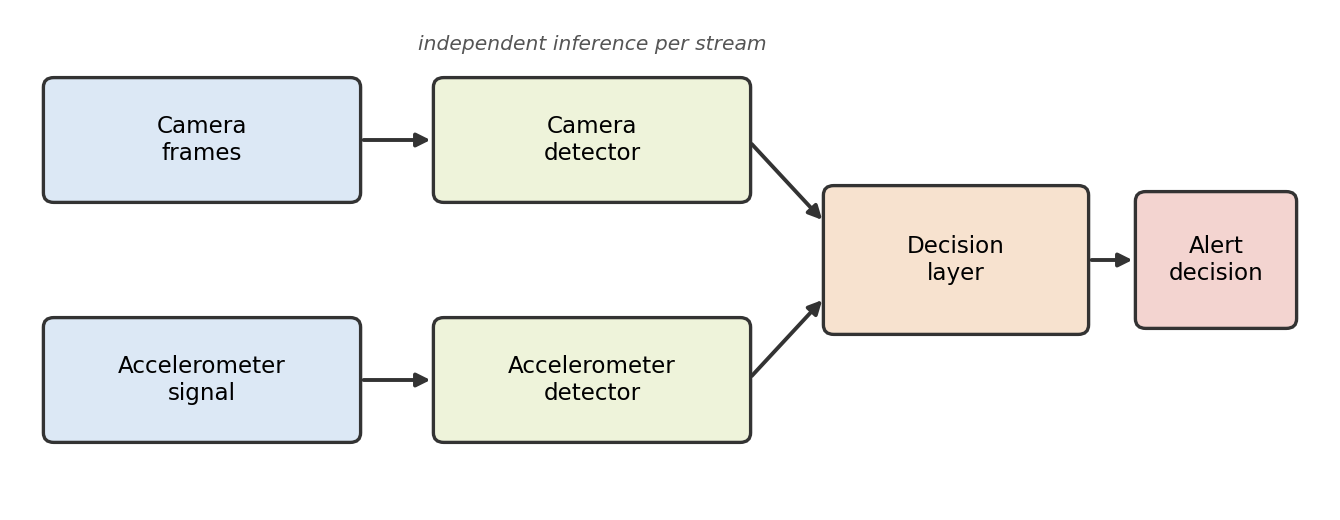
\includegraphics[width=\columnwidth]{fig_system.png}
\caption{System overview. A camera detector and an accelerometer detector are
trained and run independently. A decision layer combines their current and
recent alert outputs into a monitoring decision.}
\label{fig:system}
\end{figure}

\subsection{The Two Detectors}
Let $x_c(t)$ be the camera feature vector and $x_h(t)$ the accelerometer feature
vector at frame $t$. The camera detector and the accelerometer detector are
logistic regression models, each trained with balanced class weighting only on
its own stream, producing risk scores $C(t)$ and $H(t)$:
\begin{equation}
C(t) = \sigma(w_c^{\top} x_c(t) + b_c), \quad
H(t) = \sigma(w_h^{\top} x_h(t) + b_h)
\end{equation}
where $\sigma$ is the sigmoid. The accelerometer features are computed over a
500 millisecond window and are based on the total acceleration vector:
\begin{equation}
\mathrm{SV}(t) = \sqrt{A_x(t)^2 + A_y(t)^2 + A_z(t)^2}
\end{equation}
Window statistics of this quantity, of the per axis signals, and a slope term
form $x_h(t)$. All scores used downstream come from grouped cross validation
with whole sequences held out, so the score for any frame is produced by a model
that never trained on that sequence.

\subsection{Decision Layers}
A decision layer maps the two score streams to a binary alert decision $a(t)$.
All layers are causal. Fourteen layers are compared, in four families.

\textbf{Single sensor.} Camera Only and Accelerometer Only threshold one stream.

\textbf{Simple score combiners.} Equal Weights Fusion thresholds the equally
weighted mean $(C(t)+H(t))/2$. Max OR Fusion thresholds $\max(C(t),H(t))$, Min
Agreement Fusion thresholds $\min(C(t),H(t))$, and Product Agreement Fusion
thresholds $C(t)H(t)$. Naive Independence combines the scores under an
independence assumption:
\begin{equation}
a_{\mathrm{NI}}(t) = \mathbf{1}\!\left[\, 1 - (1-C(t))(1-H(t)) > \theta \,\right]
\end{equation}

\textbf{Rule based agreement.} For each stream a per frame alert indicator and a
persistence run length are defined recursively:
\begin{equation}
c(t) = \mathbf{1}[\,C(t) > \theta_c\,], \quad
r_c(t) = c(t)\,\bigl(r_c(t-1) + 1\bigr)
\end{equation}
where $\mathbf{1}[\cdot]$ is the indicator function. The AND rule alerts only
when both streams have persisted for at least $K$ consecutive frames, and the OR
rule when either stream has:
\begin{equation}
a_{\mathrm{AND}}(t) = \mathbf{1}[\,r_c(t) \ge K\,]\cdot\mathbf{1}[\,r_h(t) \ge K\,]
\end{equation}
\begin{equation}
a_{\mathrm{OR}}(t) = 1 - \bigl(1 - \mathbf{1}[r_c(t)\ge K]\bigr)
\bigl(1 - \mathbf{1}[r_h(t)\ge K]\bigr)
\end{equation}

\textbf{Learned fusion.} Calibrated Logistic Fusion is a calibrated logistic
model on the two current scores. The temporal learned methods use a causal
rolling mean over a window of length $L$,
\begin{equation}
\mu_C(t) = \frac{1}{L}\sum_{i=t-L+1}^{t} C(i)
\end{equation}
and a temporal feature vector combining the current scores, their product and
absolute difference, the two rolling means, and the smaller of the two means:
\begin{equation}
\begin{split}
\phi(t) = \bigl[\,&C(t),\, H(t),\, C(t)H(t),\, |C(t)-H(t)|,\\
&\mu_C(t),\, \mu_H(t),\, \min(\mu_C(t),\mu_H(t))\,\bigr]
\end{split}
\end{equation}
Temporal Logistic Fusion applies a logistic model to this vector,
\begin{equation}
a_{\mathrm{LF}}(t) = \mathbf{1}\!\left[\,\sigma(w^{\top}\phi(t) + b) > \theta\,\right]
\end{equation}
and Temporal Random Forest, Temporal Extra Trees, and Temporal
HistGradientBoosting apply tree based classifiers \cite{breiman2001} to the same
vector. All thresholds and the persistence length $K$ are tuned on the training
sequences and applied unchanged to the held out test sequences.

\section{Controlled Sensor Stress Protocol}
Clean benchmark performance can hide failure modes that matter in deployment. A
controlled stress protocol perturbs the detector score streams of the held out
test sequences while keeping the ground truth labels fixed. The protocol
emulates four failure modes: false camera evidence, false accelerometer
evidence, broadband noise on both streams, and weakened true evidence on genuine
fall frames. Stress severity ranges from 0.0, the clean condition, to 1.0, and
each severity is evaluated across ten random train and test splits by sequence.

\section{Experimental Setup}
The 70 sequences are split into training and test sets by sequence, with 65
percent of sequences used for training, repeated over ten random splits. The
detectors and all decision layer hyperparameters are fit on the training
sequences only. The primary metrics are F1, precision, recall, balanced
accuracy, and false alert rate, the last being the fraction of normal frames
incorrectly predicted as alerts:
\begin{equation}
\mathrm{FAR} = \frac{\mathrm{FP}}{\mathrm{FP} + \mathrm{TN}}, \quad
\mathrm{F1} = \frac{2\,\mathrm{P}\cdot\mathrm{R}}{\mathrm{P} + \mathrm{R}}
\end{equation}
Results are aggregated over the ten splits, and paired Wilcoxon signed rank tests
compare each method against the single stream camera detector across the ten
splits.

\section{Results}
\subsection{Detector Validation}
Evaluated by grouped cross validation across sequences, the camera detector
reaches an area under the ROC curve of 0.956 and the accelerometer detector
0.858. The camera detector is the stronger of the two. These two scores are the
inputs to every decision layer.

\subsection{Clean Leaderboard}
Table~\ref{tab:leaderboard} reports the fourteen decision layers on the co
observed benchmark under clean conditions, ranked by F1. Temporal Logistic Fusion
is the top method, with an F1 of 0.863, above the best single sensor, Camera
Only, at 0.842. Calibrated Logistic Fusion and the temporal tree models also rank
above the camera detector. The simple score combiners and the rule based methods
do not: Equal Weights Fusion (0.833) and Rule AND Tuned (0.767) both fall below
the single camera detector.

\begin{table*}[t]
\centering
\caption{Clean co observed leaderboard, mean over ten splits, ranked by F1.
Temporal Logistic Fusion leads. Rule AND Tuned has the lowest false alert rate
but the lowest recall among the fusion methods.}
\label{tab:leaderboard}
\begin{tabular}{lccccc}
\toprule
Method & F1 & Precision & Recall & Balanced Accuracy & False Alert Rate \\
\midrule
Temporal Logistic Fusion       & 0.863 & 0.895 & 0.835 & 0.891 & 0.052 \\
Temporal Random Forest         & 0.852 & 0.860 & 0.850 & 0.888 & 0.074 \\
Calibrated Logistic Fusion     & 0.851 & 0.888 & 0.824 & 0.884 & 0.056 \\
Temporal Extra Trees           & 0.850 & 0.864 & 0.843 & 0.886 & 0.071 \\
Temporal HistGradientBoosting  & 0.847 & 0.847 & 0.856 & 0.886 & 0.084 \\
Max OR Fusion                  & 0.847 & 0.858 & 0.839 & 0.881 & 0.077 \\
Naive Independence             & 0.846 & 0.843 & 0.855 & 0.883 & 0.088 \\
Camera Only                    & 0.842 & 0.890 & 0.810 & 0.878 & 0.055 \\
Equal Weights Fusion           & 0.833 & 0.798 & 0.875 & 0.876 & 0.124 \\
Product Agreement Fusion       & 0.817 & 0.826 & 0.815 & 0.860 & 0.096 \\
Min Agreement Fusion           & 0.790 & 0.800 & 0.795 & 0.840 & 0.114 \\
Rule AND Tuned                 & 0.767 & 0.926 & 0.662 & 0.816 & 0.030 \\
Accelerometer Only             & 0.741 & 0.743 & 0.767 & 0.802 & 0.162 \\
\bottomrule
\end{tabular}
\end{table*}

Two points deserve emphasis. First, the advantage of the best fusion over the
camera detector is modest, about two F1 points, although as shown below it is
statistically consistent. Second, the methods fail in interpretable ways. Equal
Weights Fusion and the OR style combiners push recall up but precision and false
alarms down. Rule AND Tuned does the opposite: it has the highest precision,
0.926, and the lowest false alert rate, 0.030, but its recall falls to 0.662
because requiring two sensors to agree misses falls that only one sensor
registered. The learned temporal fusion is the method that improves F1 without
that penalty, and it also matches or exceeds the camera detector on precision,
recall, and false alert rate.

\subsection{Statistical Significance}
Table~\ref{tab:wilcoxon} reports paired Wilcoxon signed rank tests of each fusion
method against Camera Only, on F1, at the clean condition. Temporal Logistic
Fusion improves on the camera detector in all ten of ten splits with $p$
approximately 0.002. Calibrated Logistic Fusion and Temporal Random Forest also
improve significantly, by smaller margins. Rule AND Tuned is significantly worse
than the camera detector.

\begin{table}[t]
\centering
\caption{Paired comparison against the single stream camera detector, F1, clean
condition, ten splits.}
\label{tab:wilcoxon}
\begin{tabular}{lccc}
\toprule
Method vs Camera Only & $\Delta$ F1 & Wins / Losses & Wilcoxon $p$ \\
\midrule
Temporal Logistic Fusion    & $+0.021$ & 10 / 0 & 0.002 \\
Temporal Random Forest      & $+0.010$ & 8 / 2  & 0.027 \\
Calibrated Logistic Fusion  & $+0.009$ & 10 / 0 & 0.002 \\
Temporal Extra Trees        & $+0.008$ & 8 / 2  & 0.084 \\
Naive Independence          & $+0.004$ & 7 / 3  & 0.625 \\
Equal Weights Fusion        & $-0.009$ & 2 / 8  & 0.160 \\
Rule AND Tuned              & $-0.075$ & 1 / 9  & 0.004 \\
\bottomrule
\end{tabular}
\end{table}

\subsection{Robustness Under Sensor Stress}
Figure~\ref{fig:f1stress} shows F1 as the stress severity increases. Temporal
Logistic Fusion is the top method at every stress level, and the paired Wilcoxon
advantage over Camera Only holds at every level, with $p$ approximately 0.002 and
ten of ten winning splits at most levels. The margin stays in the range of two to
three F1 points across the full stress range. Both the best fusion and the camera
detector are fairly flat under this protocol, so the result is best described as
a consistent fixed gap rather than a difference in degradation rate.

\begin{figure}[t]
\centering
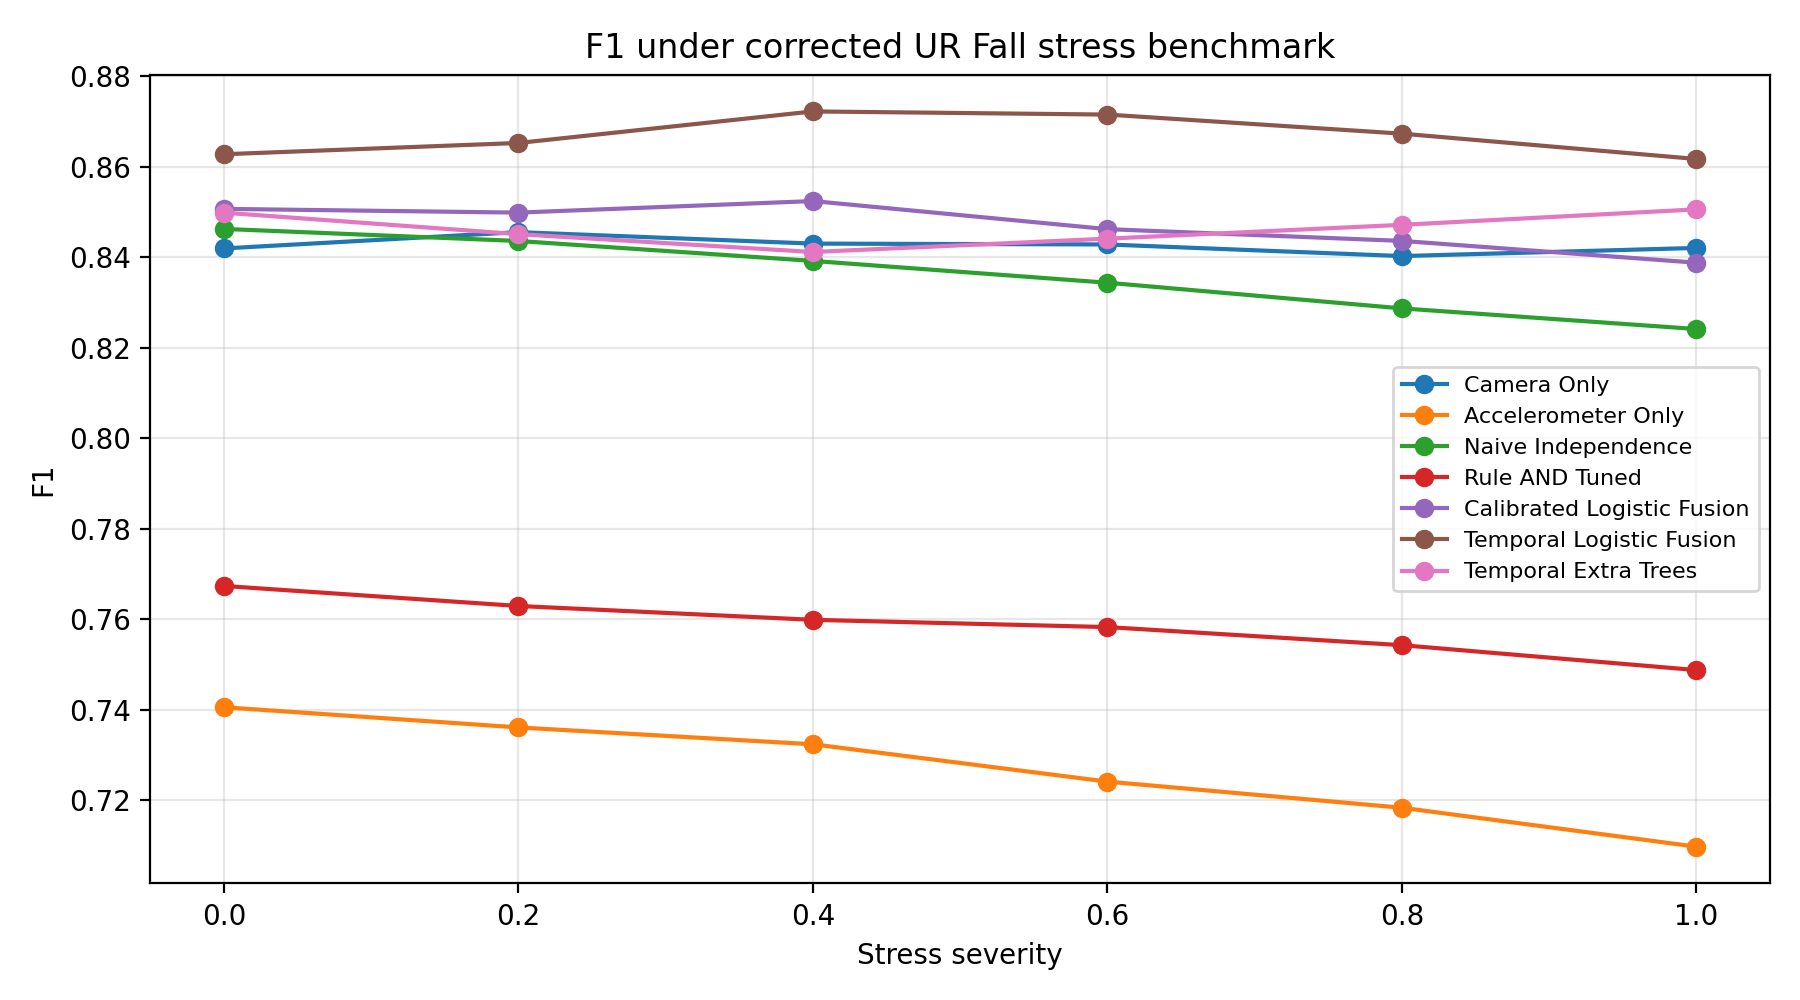
\includegraphics[width=\columnwidth]{fig_f1_stress.png}
\caption{F1 under increasing sensor stress. Temporal Logistic Fusion leads at
every stress level. The simple combiners and the rule based fusion remain below
the camera detector.}
\label{fig:f1stress}
\end{figure}

Figure~\ref{fig:farstress} shows the false alert rate. Rule AND Tuned keeps the
lowest false alert rate throughout, a consequence of its strict agreement
requirement, while paying for it in recall and F1. Temporal Logistic Fusion has a
false alert rate close to the camera detector, and the paired difference between
the two is small and mostly not significant. So the learned temporal fusion
improves F1 over the camera detector without a meaningful false alarm penalty,
whereas the equal weight and OR style combiners raise false alarms substantially.

\begin{figure}[t]
\centering
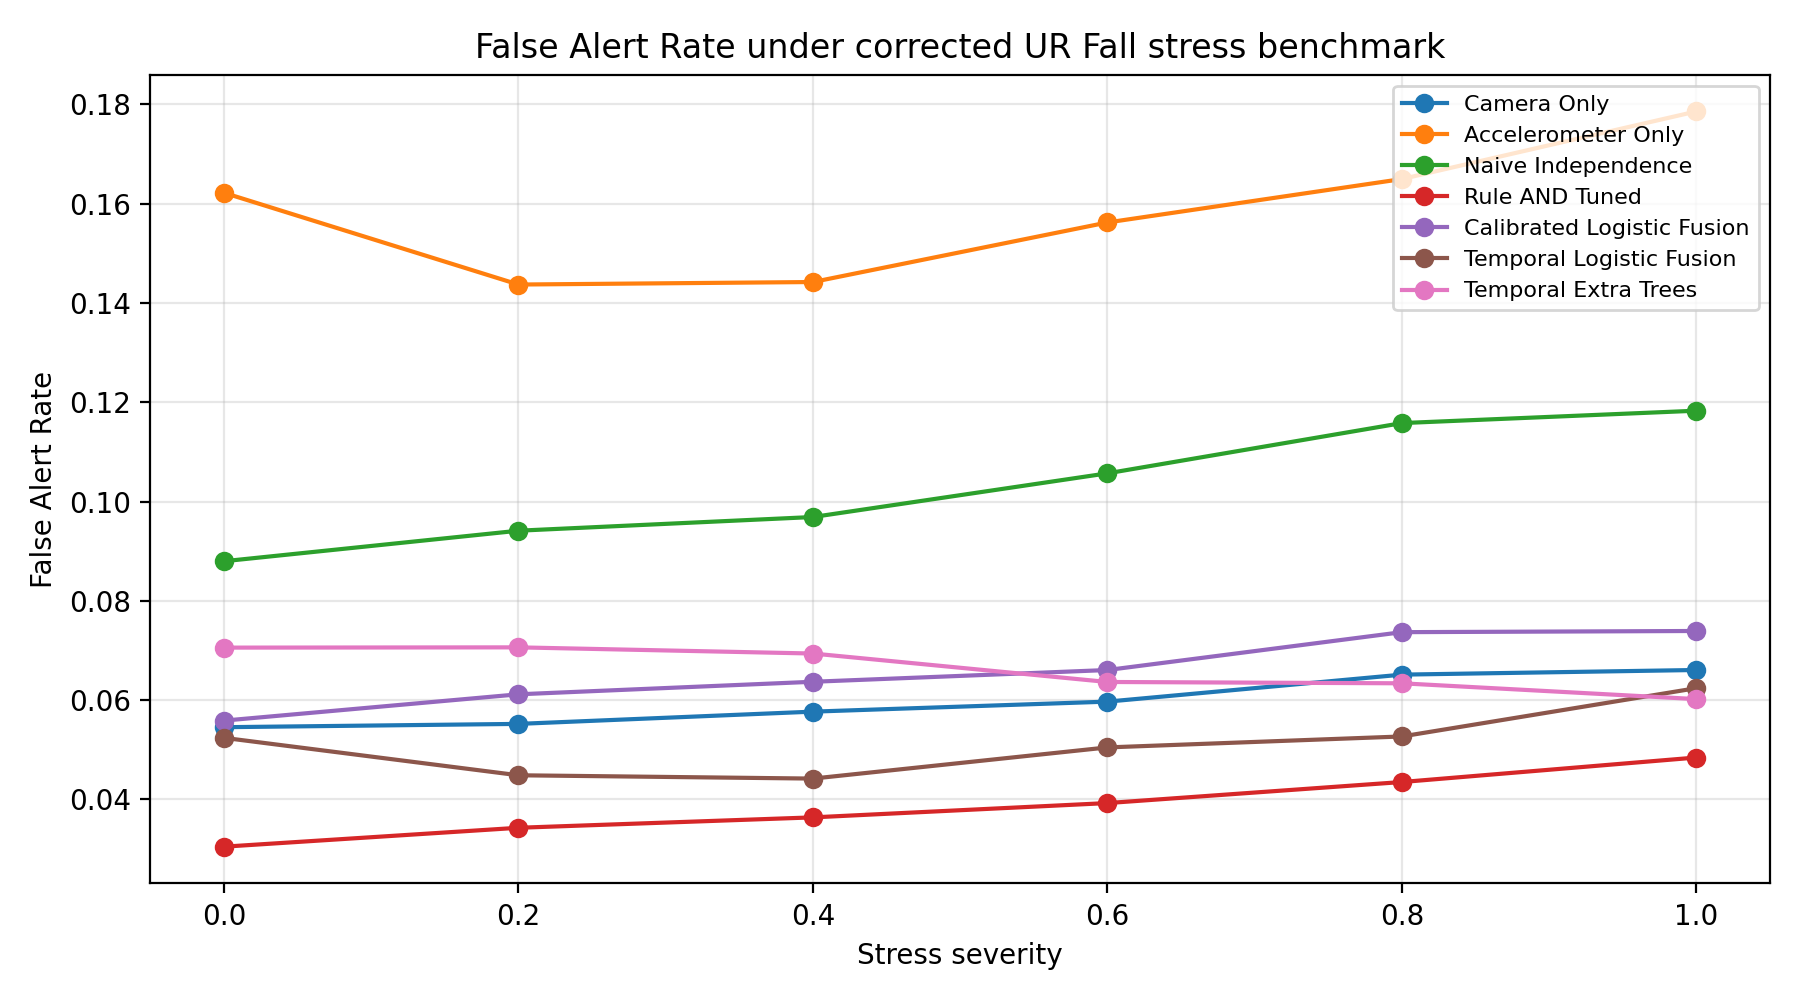
\includegraphics[width=\columnwidth]{fig_far_stress.png}
\caption{False alert rate under increasing sensor stress.}
\label{fig:farstress}
\end{figure}

\section{Discussion}
The results support a measured and honest claim. On co observed camera and
accelerometer fall data, a learned temporal decision layer improves on the best
single sensor, and a hand designed or equal weight decision layer does not. The
improvement is small, about two to three F1 points, but it is statistically
significant and consistent: Temporal Logistic Fusion beats the camera detector in
all or almost all of ten paired splits at every stress level. A small gain that
holds across ten splits and six stress levels is a real effect, and it should be
presented as small and real, not as large.

The shape of the result is informative. The simple score combiners trade recall
against precision but do not improve the balance: equal weight averaging and OR
style combiners raise recall and false alarms together, while the strict AND rule
raises precision and suppresses false alarms at a heavy cost in recall. The
learned temporal fusion is the only family that improves F1 without that penalty,
because it can weight the two streams and their recent history rather than
applying a fixed rule. This is why the contribution is specifically a learned
temporal decision layer, and not the agreement rule: the rule, evaluated
honestly, finishes below the single camera detector.

For deployment the practical reading is that the choice of decision layer should
follow the priority. If balanced detection accuracy is the goal, the learned
temporal fusion is the best option tested. If the overriding goal is to minimize
false alarms, the strict AND rule delivers the lowest false alert rate, at a real
cost in missed falls. There is no method here that is best on every metric, and
the paper does not claim one.

\section{Limitations and Threats to Validity}
\textbf{Modest effect size.} The improvement of the best fusion over the best
single sensor is small. It is statistically robust across splits and stress
levels, but it is not a large gain, and the paper does not present it as one.

\textbf{Simulated falls.} The falls in the dataset were performed by healthy
volunteers. Real falls by older adults differ in dynamics, and performance may
not transfer directly. This limitation is shared by most public fall detection
datasets.

\textbf{Single dataset.} The evaluation uses one co observed dataset. The
conclusions should be confirmed on additional co observed multimodal data.

\textbf{Camera representation.} The camera branch uses extracted depth map
features rather than a state of the art video encoder. This keeps the comparison
controlled but does not claim best possible visual detection.

\textbf{Physiological extension not validated.} The decision layer is agnostic to
the second modality. A natural extension replaces the accelerometer stream with a
physiological vital sign stream for health deterioration detection. No public
dataset currently provides video synchronized with real vital signs during fall
or health deterioration events, so that extension cannot yet be validated on co
observed data, and collecting such a dataset is important future work.

\textbf{Stress protocol.} The stress protocol perturbs detector scores to emulate
sensor failure. It is a controlled abstraction, not a substitute for real
deployment evaluation.

\section{Reproducibility}
The evaluation pipeline is implemented as a self contained notebook that
downloads the UR Fall Detection Dataset, builds the per frame co observed events,
runs an explicit label sanity check, trains the two detectors, and runs every
decision layer and the stress protocol across ten splits. The UR Fall Detection
Dataset is publicly available for academic use. The notebook, the feature
extraction code, the decision layer implementations, the stress protocol, and the
figure and table scripts are released publicly at
\textcolor{red}{[insert public repository link before submission]}, which is
necessary because the co observed benchmark construction and the stress protocol
are specific to this work.

\section{Conclusion}
This paper evaluated decision level fusion for home fall monitoring on co
observed data, in which a camera and a body worn accelerometer recorded the same
falls at the same time. Across a fourteen method leaderboard, a learned temporal
fusion, a logistic model over causal temporal features of the two detector
streams, was the strongest method, improving F1 over the best single sensor from
0.842 to 0.863. The improvement is modest but statistically significant and
consistent across ten splits and six stress levels, and it comes without a
meaningful false alarm penalty. Simpler fusion strategies, including a hand
designed rule based agreement rule and equal weight score averaging, did not beat
the single sensor. The honest summary is that a learned temporal decision layer
gives a small, consistent, real improvement, while simpler decision layers do
not. Future work should evaluate additional co observed multimodal datasets and,
if suitable data can be collected, extend the evaluation to a physiological vital
sign stream.

\begin{thebibliography}{14}
\bibitem{baltrusaitis2019} T. Baltrusaitis, C. Ahuja, and L. P. Morency,
``Multimodal machine learning: A survey and taxonomy,'' \emph{IEEE Trans.
Pattern Anal. Mach. Intell.}, 2019.
\bibitem{atrey2010} P. K. Atrey, M. A. Hossain, A. El Saddik, and M. S.
Kankanhalli, ``Multimodal fusion for multimedia analysis: A survey,''
\emph{Multimedia Systems}, 2010.
\bibitem{mubashir2013} M. Mubashir, L. Shao, and L. Seed, ``A survey on fall
detection: Principles and approaches,'' \emph{Neurocomputing}, 2013.
\bibitem{rougier2007} C. Rougier, J. Meunier, A. St Arnaud, and J. Rousseau,
``Fall detection from human shape and motion history using video
surveillance,'' in \emph{Proc. IEEE AINA Workshops}, 2007.
\bibitem{kwolek2014} B. Kwolek and M. Kepski, ``Human fall detection on embedded
platform using depth maps and wireless accelerometer,'' \emph{Computer Methods
and Programs in Biomedicine}, 2014.
\bibitem{kepski2018} M. Kepski and B. Kwolek, ``Event driven system for fall
detection using body worn accelerometer and depth sensor,'' \emph{IET Computer
Vision}, 2018.
\bibitem{nunez2017} A. Nunez Marcos, G. Azkune, and I. Arganda Carreras,
``Vision based fall detection with convolutional neural networks,'' \emph{Wireless
Communications and Mobile Computing}, 2017.
\bibitem{martinez2019} L. Martinez Villasenor et al., ``UP Fall detection
dataset: A multimodal approach,'' \emph{Sensors}, 2019.
\bibitem{dietterich2000} T. G. Dietterich, ``Ensemble methods in machine
learning,'' in \emph{Multiple Classifier Systems}, 2000.
\bibitem{platt1999} J. Platt, ``Probabilistic outputs for support vector
machines and comparisons to regularized likelihood methods,'' in \emph{Advances
in Large Margin Classifiers}, 1999.
\bibitem{breiman2001} L. Breiman, ``Random forests,'' \emph{Machine Learning},
2001.
\bibitem{pedregosa2011} F. Pedregosa et al., ``Scikit learn: Machine learning in
Python,'' \emph{Journal of Machine Learning Research}, 2011.
\bibitem{guo2017} C. Guo, G. Pleiss, Y. Sun, and K. Q. Weinberger, ``On
calibration of modern neural networks,'' in \emph{Proc. ICML}, 2017.
\bibitem{moody2001} G. B. Moody and R. G. Mark, ``The impact of the MIT BIH
arrhythmia database,'' \emph{IEEE Eng. Med. Biol. Mag.}, 2001.
\end{thebibliography}

\end{document}
